\documentclass[aspectratio=169]{beamer}
\useoutertheme[progressbar=frametitle]{metropolis}
\useinnertheme{metropolis}


\definecolor{nabgray}{rgb}{0.6,0.59,0.61}
\usecolortheme[named=nabgray]{structure}

\usepackage{tikz}
\usepackage[utf8]{inputenc}
\usepackage[portuguese]{babel}

\usepackage{smartdiagram}
\usepackage{qtree}
\usepackage{verbatim}
\usepackage{svg}
\usepackage{graphicx}
\usepackage{color}

\definecolor{lightgray}{rgb}{0.95, 0.95, 0.95}
\definecolor{darkgray}{rgb}{0.4, 0.4, 0.4}
%\definecolor{purple}{rgb}{0.65, 0.12, 0.82}
\definecolor{editorGray}{rgb}{0.95, 0.95, 0.95}
\definecolor{editorOcher}{rgb}{1, 0.5, 0} % #FF7F00 -> rgb(239, 169, 0)
\definecolor{editorGreen}{rgb}{0, 0.5, 0} % #007C00 -> rgb(0, 124, 0)
\definecolor{orange}{rgb}{1,0.45,0.13}
\definecolor{olive}{rgb}{0.17,0.59,0.20}
\definecolor{brown}{rgb}{0.69,0.31,0.31}
\definecolor{purple}{rgb}{0.38,0.18,0.81}
\definecolor{lightblue}{rgb}{0.1,0.57,0.7}
\definecolor{lightred}{rgb}{1,0.4,0.5}
\usepackage{upquote}
\usepackage{listings}
\lstset{language=java,
	basicstyle=\footnotesize\ttfamily,
	keywordstyle=\footnotesize\color{blue}\ttfamily,
	escapeinside={<@}{@>}
}
\lstdefinelanguage{Kotlin}{
	comment=[l]{//},
	commentstyle={\color{gray}\ttfamily},
	emph={delegate, filter, first, firstOrNull, forEach, lazy, map, mapNotNull, println, return@},
	emphstyle={\color{purple}},
	identifierstyle=\color{black},
	keywords={abstract, actual, as, as?, break, by, class, companion, continue, data, do, dynamic, else, enum, expect, false, final, for, fun, get, if, import, in, interface, internal, is, null, object, override, package, private, public, return, set, super, suspend, this, throw, true, try, typealias, val, var, vararg, when, where, while},
	keywordstyle={\color{lightblue}\bfseries},
	morecomment=[s]{/*}{*/},
	morestring=[b]",
	morestring=[s]{"""*}{*"""},
	ndkeywords={@Inject, @Deprecated, @JvmField, @JvmName, @JvmOverloads, @JvmStatic, @JvmSynthetic, Array, Byte, Double, Float, Int, Integer, Iterable, Long, Runnable, Short, String},
	ndkeywordstyle={\color{orange}\bfseries},
	sensitive=true,
	stringstyle={\color{olive}\ttfamily},
}


\usebackgroundtemplate%
{%
	
\includegraphics[width=\paperwidth]{Images/Contenido.png}%
}


\title{O estado atual do Kotlin no backend}
\author{Víctor Orozco - Nabenik}
\institute{@tuxtor}
\date{\today}

\begin{document}
{
    \usebackgroundtemplate{
\includegraphics[width=\paperwidth]{Images/portada}}
    \setbeamercolor{frametitle}{fg=red}
    \usebeamercolor[fg]{normal text}
    \frame{\titlepage}
}

\begin{frame}[fragile]{¿Java?}
\begin{columns}
    \begin{column}{0.5\textwidth}
        \begin{itemize}
            \item Linguagem (Java 16)
            \item OpenJDK (Java Virtual Machine)
            \item Bibliotecas/API (Java Classpath)
        \end{itemize}
    \end{column}
    \begin{column}{0.5\textwidth}  %%<--- here
        \begin{figure}
            \centering
            
\includegraphics[width=0.4\linewidth]{Images/java}
        \end{figure}
    \end{column}
\end{columns}

As três juntas são a plataforma Java
\end{frame}

\begin{frame}[fragile]{Java no Android}

    \begin{columns}
        \begin{column}{0.5\textwidth}
            \begin{itemize}
                \item Linguagem (Java 7 + Lambdas + DateTime)
                \item ART/Dalvik
                \item Bibliotecas/API (Java+Google Classpath)
            \end{itemize}
        \end{column}
        \begin{column}{0.5\textwidth}  %%<--- here
            \begin{figure}
                \centering
                
\includegraphics[width=0.4\linewidth]{Images/java}
            \end{figure}
        \end{column}
    \end{columns}


\end{frame}


\begin{frame}[fragile]{Kotlin}
    \begin{columns}
        \begin{column}{0.5\textwidth}
            \begin{itemize}
                \item Linguagem (Kotlin)
                \item OpenJDK (Java Virtual Machine)
                \item Bibliotecas/API (Java Classpath)
                \item kotlin-stdlib
            \end{itemize}
        \end{column}
        \begin{column}{0.5\textwidth}  %%<--- here
            \begin{figure}
                \centering
                
\includegraphics[width=0.4\linewidth]{Images/kotlin}
            \end{figure}
        \end{column}
    \end{columns}
\end{frame}


{
    \usebackgroundtemplate{
\includegraphics[width=\paperwidth]{Images/separador}}
    \setbeamercolor{normal text}{fg=white}
    \setbeamercolor{frametitle}{fg=red}
    \usebeamercolor[fg]{normal text}
    \section{Modelos de desenvolvimento}
}


\begin{frame}[fragile]{Desenvolvimento backend Java no 2021 - Concorrência}
Thread based -e.g. EJB, CDI, JAX-RS-
\begin{lstlisting}[language=Java]
@Inject
SayService say;

@GET
@Produces(MediaType.TEXT_PLAIN)
public String hello() {
    return say.hello();
}
\end{lstlisting}

JakartaEE/MicroProfile
\end{frame}


\begin{frame}[fragile]{Desenvolvimento backend Java no 2021 - Concorrência}
Reactive based -e.g. Async JAX-RS, Spring WebFlux, Actors, Verticles-
\begin{lstlisting}[language=Java]
public class Server extends AbstractVerticle {
  public void start() {
    vertx.createHttpServer().requestHandler(req -> {
      req.response()
        .putHeader("content-type", "text/plain")
        .end("Hello from Vert.x!");
    }).listen(8080);
  }
}
\end{lstlisting}
Vert.x
\end{frame}


\begin{frame}{Desenvolvimento backend Java no 2021 - Arquitetura}

\begin{columns}
\begin{column}{0.5\textwidth}
\begin{itemize}
	\item Monólito
    \item Microserviço
    \item Micromonolito
\end{itemize}
\end{column}
\begin{column}{0.5\textwidth}  %%<--- here
\begin{figure}
	\centering
	
\includegraphics[width=0.9\linewidth]{Images/micromonolito.png}
\end{figure}
\end{column}
\end{columns}

\end{frame}


\begin{frame}{Desenvolvimento backend Java no 2021 - Runtime}

\begin{columns}
\begin{column}{0.5\textwidth}
"Simples/DIY"
\begin{itemize}
\item Servlet based -e.g. Tomcat, Jetty-
\item Custom I/O -e.g. Undertow, Netty, Vert.x-
\end{itemize}
\end{column}
\begin{column}{0.5\textwidth}  %%<--- here
\begin{figure}
	\centering
	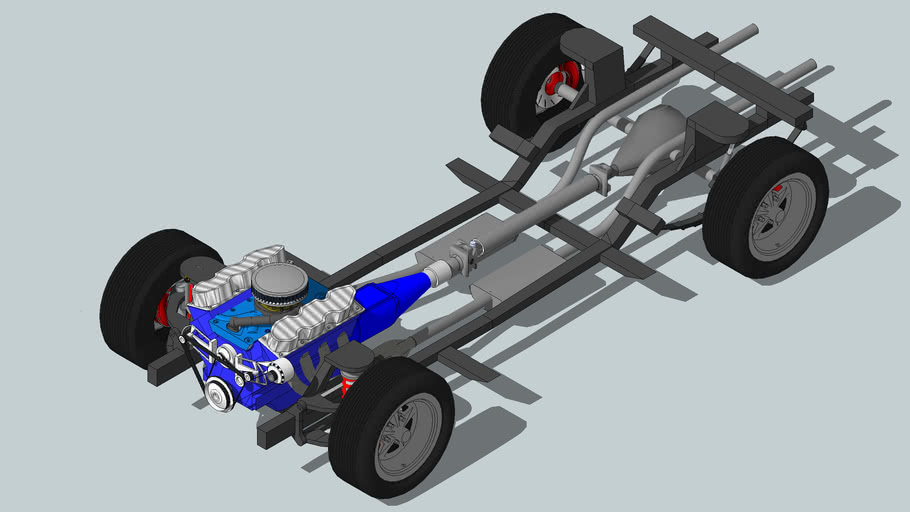
\includegraphics[width=0.9\linewidth]{Images/chassis}
\end{figure}
\end{column}
\end{columns}

\end{frame}


\begin{frame}{Desenvolvimento backend Java no 2021 - Runtime/Framework}

\begin{columns}
\begin{column}{0.5\textwidth}
"Micro"
\begin{itemize}
\item Custom micro -e.g. Jooby, Spark, Javalin, Helidon SE-
\item MicroProfile based -e.g. Quarkus, Helidon-
\item Micronaut
\item Spring Boot
\end{itemize}
\end{column}
\begin{column}{0.5\textwidth}  %%<--- here
\begin{figure}
	\centering
	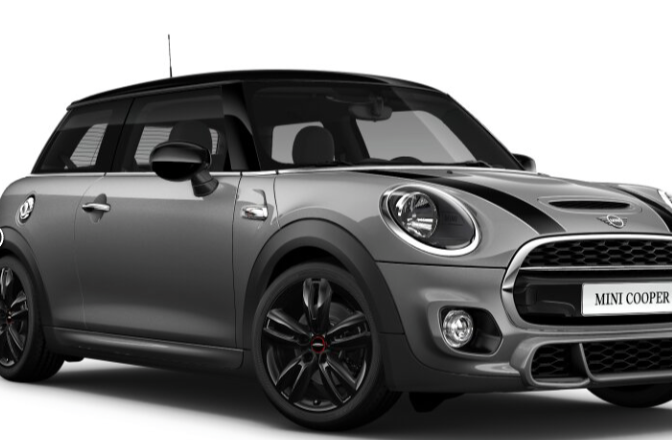
\includegraphics[width=0.9\linewidth]{Images/cooper}
\end{figure}
\end{column}
\end{columns}

\end{frame}

\begin{frame}{Desenvolvimento backend Java no 2021}

\begin{columns}
\begin{column}{0.5\textwidth}

"Complexo"
\begin{itemize}
\item Java EE/Jakarta EE -e.g. JBoss, WebSphere Liberty-
\item Spring
\item Akka
\end{itemize}
\end{column}
\begin{column}{0.5\textwidth}  %%<--- here
\begin{figure}
	\centering
	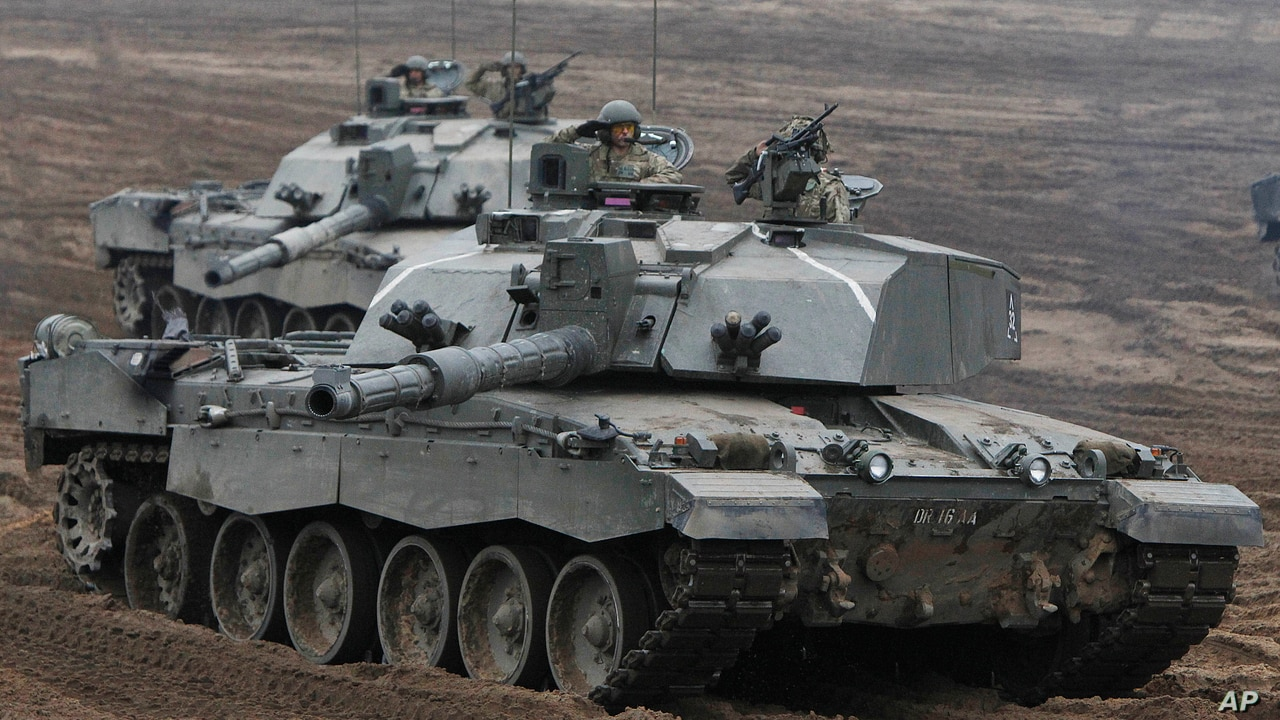
\includegraphics[width=0.9\linewidth]{Images/tank}
\end{figure}
\end{column}
\end{columns}

\end{frame}

\begin{frame}{Arquiteto Java no ano 2021}

\begin{exampleblock}{Arquiteto Java}
O cara que tem que decidir entre pegar um framework pronto \textit{complexo} ou pegar um runtime \textit{ligero} e criar a estrutura toda -i.e Bibliotecas, estilo arquitetural, SCM (Maven)-.\\


O cara que tem que decidir entre chatear os dev Java tradicionais no modelo de desenvolvimento Async ou chatear os desenvolvedores Kotlin por não aproveitar os Coroutines que nem no Android.\\

O cara que tem que avaliar dar o pulo para o Kotlin conservando os stacks tradicionais.

\end{exampleblock}
\end{frame}

\begin{frame}{Arquiteto Java no ano 2021}

\begin{exampleblock}{Arquiteto Java}
O cara que vai ser odiado por não dar o pulo para JavaScript só pela vontade de re-escreber a base de código que vem fazendo succeso há 15 anos
\end{exampleblock}
\end{frame}

{
    \usebackgroundtemplate{
\includegraphics[width=\paperwidth]{Images/separador}}
    \setbeamercolor{normal text}{fg=white}
    \setbeamercolor{frametitle}{fg=red}
    \usebeamercolor[fg]{normal text}
    \section{Kotlin no backend}
}


\begin{frame}{Kotlin no backend - Fatos}

\begin{exampleblock}{Fato \#1}
Todo framework Java pode virar framework Kotlin. Mas nem todo framework Java e testado no Kotlin.
\end{exampleblock}
\end{frame}

\begin{frame}{Kotlin no backend - Fatos}
\begin{figure}
	\centering
	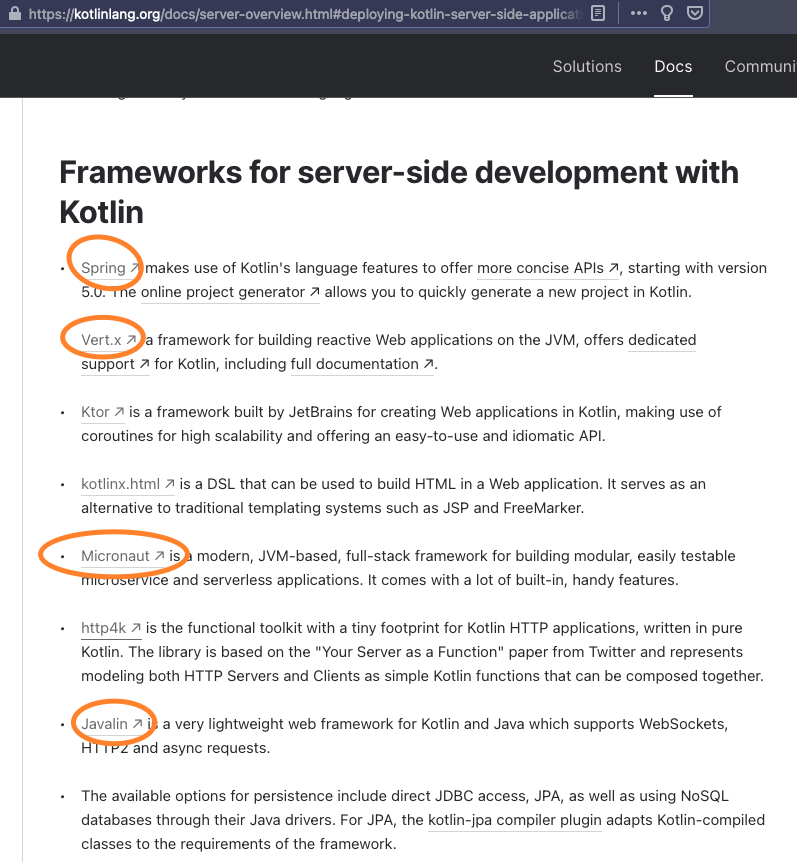
\includegraphics[width=0.55\linewidth]{Images/fwkotlin}
\end{figure}
\end{frame}

\begin{frame}{Kotlin no backend - Fatos}

Frameworks com suporte oficial

\begin{itemize}
\item
\end{itemize}

\end{frame}

\begin{frame}{Kotlin no backend - Fatos}

\begin{exampleblock}{Fato \#2}
Geralmente o problema são os annotation processors -e.g. Lombok-, muitos são feitos para o Java
\end{exampleblock}
\end{frame}

\begin{frame}{Kotlin no backend - Fatos}

\begin{exampleblock}{Fato \#3}
O ecosistema Kotlin esta criando Frameworks Kotlin-first/Kotlin-exclusive
\end{exampleblock}
\end{frame}

\begin{frame}[fragile]{Kotlin no backend - Fatos}
Reactive based - DIY
\begin{lstlisting}[language=Kotlin]
fun HelloWorld(): HttpHandler {
    return routes("/" bind GET to { Response(OK).body("hello world!") })
}
\end{lstlisting}
Http4k
\end{frame}

\begin{frame}[fragile]{Kotlin no backend - Fatos}
Reactive based - Micro
\begin{lstlisting}[language=Kotlin]
fun main(args: Array<String>) {
    embeddedServer(Netty, 8080) {
        routing {
            get("/") {
                call.respondText("Hello, world!", ContentType.Text.Html)
            }
        }
    }.start(wait = true)
}
\end{lstlisting}
Ktor
\end{frame}


\begin{frame}{Java - Dying since 1995}
\begin{columns}
\begin{column}{0.5\textwidth}
\begin{itemize}
	\item Spring Boot, Micronaut, MicroProfile, GraalVM . . .
	\item Raw performance (Beam, Spark, Hadoop)
	\item Tooling - IDE, Maven, Drivers RDBMS
	\item JVM - (Twitter, Alibaba, Spotify, etc.)
	\item OpenJDK
\end{itemize}
\end{column}
\begin{column}{0.5\textwidth}  %%<--- here
\begin{figure}
	\centering
	
\includegraphics[width=0.4\linewidth]{Images/java}
\end{figure}
\end{column}
\end{columns}
\end{frame}

\begin{frame}{Kotlin}
\begin{columns}

	\begin{column}{0.5\textwidth}
		Vantagens
		\begin{itemize}
			\item Código conciso enquanto você conheça as convenções
			\item Java inter-op
			\item Backend para desenvolvedores Android
			\item Uma nova forma de virar \textit{fullStack}
		\end{itemize}
	\end{column}
	\begin{column}{0.5\textwidth}
		Desvantagens
		\begin{itemize}
			\item IntelliJ IDEA Ultimate
			\item Precisa tempo para aprender e virar produtivo
			\item Tempo de compilação
			\item Thread-managed vs Co-routines
			\item Amber, Loom, Valhalla, Panama (Java 18?)
		\end{itemize}
	\end{column}
\end{columns}
\end{frame}

{
    \usebackgroundtemplate{
\includegraphics[width=\paperwidth]{Images/separador}}
    \setbeamercolor{normal text}{fg=white}
    \setbeamercolor{frametitle}{fg=red}
    \usebeamercolor[fg]{normal text}
    \section{Projeto tradicional com Kotlin}
}





\begin{frame}{Projeto Java so que não}
\begin{enumerate}
	\item Maven
	\item Dependencias (MicroProfile, Jakarta EE, Arquillian, JUnit, . . .)
	\item Maven plugin (maven-compiler-plugin)
	\item Kotlin plugin (kotlin-maven-plugin)
\end{enumerate}
\end{frame}


\begin{frame}[fragile]{Eclipse MicroProfile com Payara 5}
\begin{lstlisting}
<dependency>
	<groupId>org.eclipse.microprofile</groupId>
	<artifactId>microprofile</artifactId>
	<type>pom</type>
	<version>3.2</version>
	<scope>provided</scope>
</dependency>
\end{lstlisting}
\end{frame}


\begin{frame}[fragile]{Kotlin with Maven - Dependency}
\begin{lstlisting}[language=XML]
<dependency>
	<groupId>org.jetbrains.kotlin</groupId>
	<artifactId>kotlin-stdlib-jdk8</artifactId>
	<version>${kotlin.version}</version>
</dependency>
\end{lstlisting}
\end{frame}

\begin{frame}[fragile]{Kotlin with Maven - maven-compiler-plugin}
\begin{lstlisting}[language=xml,
basicstyle=\tiny, %or \small or \footnotesize etc.
]
<execution>
	<id>default-compile</id>
	<phase>none</phase>
</execution>
<execution>
	<id>default-testCompile</id>
	<phase>none</phase>
</execution>
<execution>
	<id>java-compile</id>
	<phase>compile</phase>
	<goals> <goal>compile</goal> </goals>
</execution>
<execution>
	<id>java-test-compile</id>
	<phase>test-compile</phase>
	<goals> <goal>testCompile</goal> </goals>
</execution>
\end{lstlisting}
\end{frame}


\begin{frame}[fragile]{Kotlin with Maven - kotlin-maven-plugin}
\begin{lstlisting}[
basicstyle=\tiny, %or \small or \footnotesize etc.
]
<compilerPlugins>
<plugin>all-open</plugin>
</compilerPlugins>
...
<option>all-open:annotation=javax.ws.rs.Path</option>
<option>all-open:annotation=javax.enterprise.context.RequestScoped</option>
<option>all-open:annotation=javax.enterprise.context.SessionScoped</option>
<option>all-open:annotation=javax.enterprise.context.ApplicationScoped</option>
<option>all-open:annotation=javax.enterprise.context.Dependent</option>
<option>all-open:annotation=javax.ejb.Singleton</option>
<option>all-open:annotation=javax.ejb.Stateful</option>
<option>all-open:annotation=javax.ejb.Stateless</option>
\end{lstlisting}

Ideia geral: As anotações Java viram open classes por causa do proxy-classes metapadrão
\end{frame}


\begin{frame}{Kotlin + Jakarta EE + MicroProfile  - Demo}

\begin{itemize}
	\item Kotlin 1.3
	\item Libraries - SLF4J, Flyway, PostgreSQL
	\item Jakarta EE 8 - EJB, JPA
	\item MicroProfile - CDI, JAX-RS, MicroProfile Config
	\item Testing - Arquillian, JUnit, Payara Embedded
\end{itemize}


\normalsize  \url{https://dzone.com/articles/the-state-of-kotlin-for-jakarta-eemicroprofile-tra}\\
\normalsize  \url{https://github.com/tuxtor/integrum-ee}
\end{frame}

\begin{frame}{Kotlin + Jakarta EE + MicroProfile  - Demo}
\begin{figure}
	\centering
	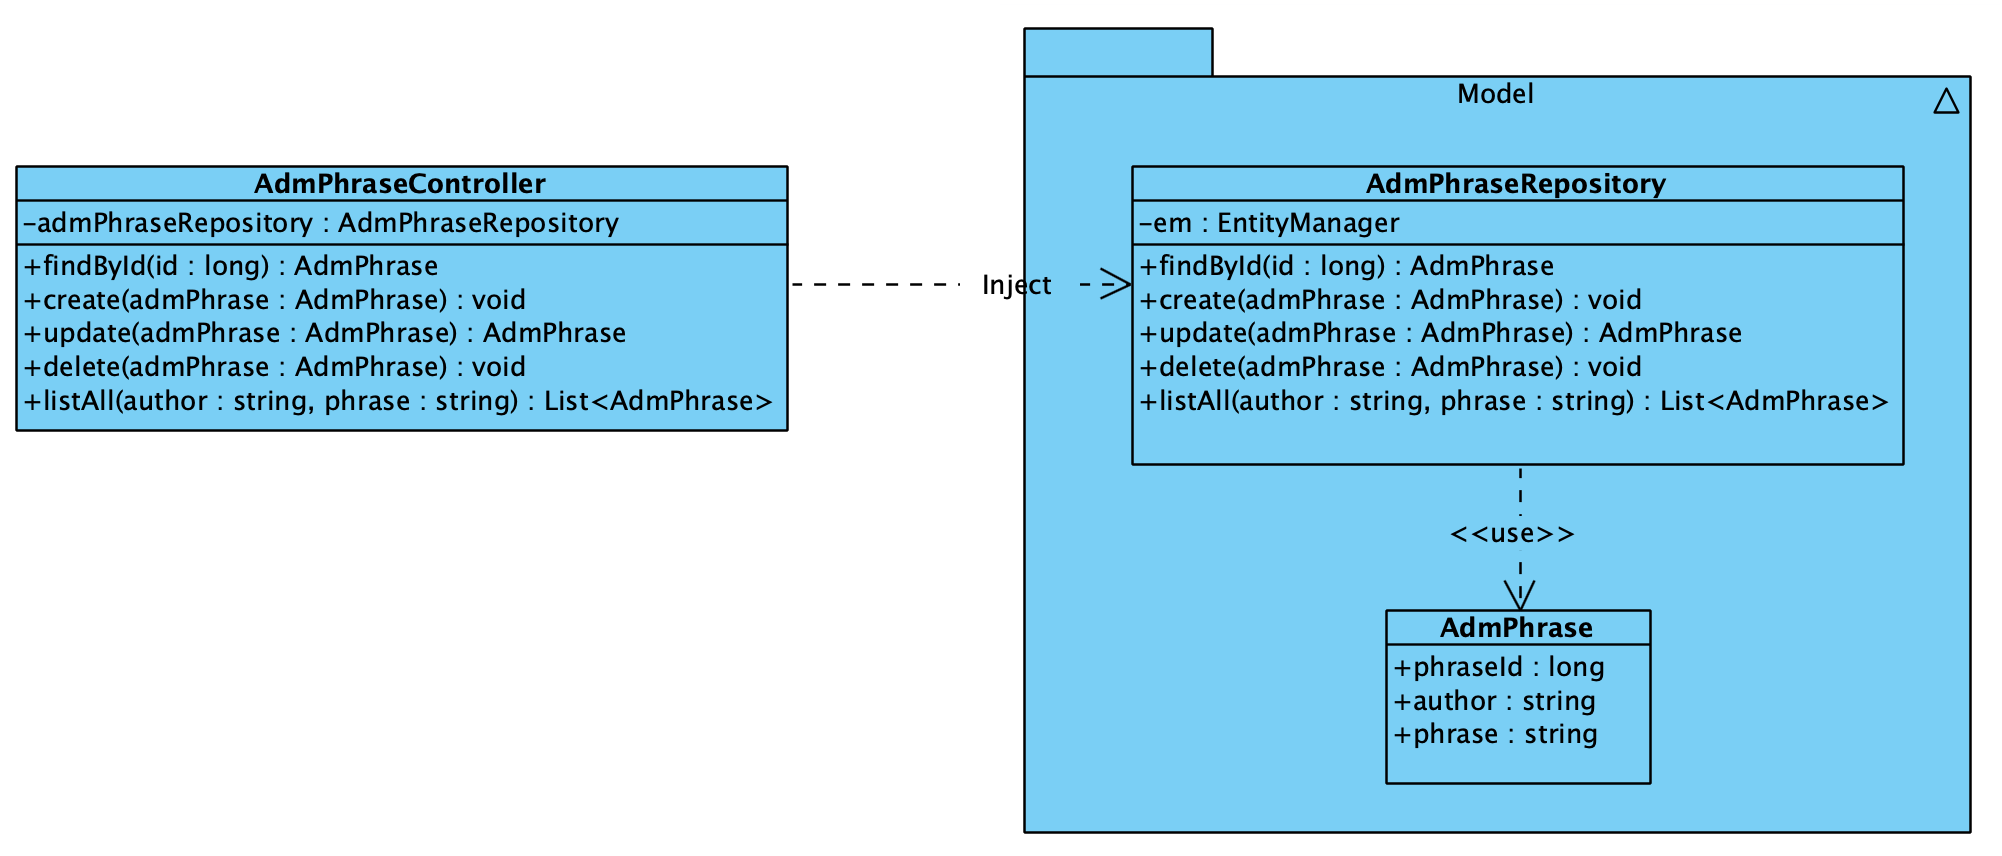
\includegraphics[width=\linewidth]{Images/integrum-ee}
\end{figure}
\end{frame}


\begin{frame}[fragile]{Kotlin - JPA entity}
\begin{lstlisting}[language=Kotlin]
@Entity
@Table(name = "adm_phrase")
@TableGenerator(...)
data class AdmPhrase(
	@Id
	@GeneratedValue(strategy = GenerationType.TABLE,
		generator = "admPhraseIdGenerator")
	@Column(name = "phrase_id")
	var phraseId:Long? = null,
	var author:String = "",
	var phrase:String = ""
)
\end{lstlisting}
Data Clases, Nullable Types
\end{frame}

\begin{frame}[fragile]{Kotlin - CDI Repository}
\begin{lstlisting}[language=Kotlin]
@RequestScoped
class AdmPhraseRepository {

	@Inject
	private lateinit var em:EntityManager

	...

}
\end{lstlisting}
Lateinit (nullable type)
\end{frame}

\begin{frame}[fragile]{Kotlin - CDI Repository}
\begin{lstlisting}[language=Kotlin]
fun create(admPhrase:AdmPhrase) = em.persist(admPhrase)

fun update(admPhrase:AdmPhrase) = em.merge(admPhrase)

fun findById(phraseId: Long) =
em.find(AdmPhrase::class.java, phraseId)

fun delete(admPhrase: AdmPhrase) = em.remove(admPhrase)
. . .
\end{lstlisting}
Single expression functions (One line methods)
\end{frame}

\begin{frame}[fragile]{Kotlin - CDI Repository}
\begin{lstlisting}[language=Kotlin]
fun listAll(author: String, phrase: String):
	List<AdmPhrase> {

	val query = """SELECT p FROM AdmPhrase p
	where p.author LIKE :author
	and p.phrase LIKE :phrase
	"""

	return em.createQuery(query, AdmPhrase::class.java)
		.setParameter("author", "%$author%")
		.setParameter("phrase", "%$phrase%")
		.resultList
}
\end{lstlisting}
Multiline string
\end{frame}

\begin{frame}[fragile]{Kotlin - JAX-RS Controllers}
\begin{lstlisting}[language=Kotlin, basicstyle=\scriptsize]
@Path("/phrases")
@Produces(MediaType.APPLICATION_JSON)
@Consumes(MediaType.APPLICATION_JSON)
class AdmPhraseController{

	@Inject
	private lateinit var admPhraseRepository: AdmPhraseRepository

	@Inject
	private lateinit var logger: Logger
	...

}
\end{lstlisting}
\end{frame}

\begin{frame}[fragile]{Kotlin - JAX-RS Controller}
\begin{lstlisting}[language=Kotlin, basicstyle=\scriptsize]

@GET
fun findAll(
@QueryParam("author") @DefaultValue("%") author: String,
@QueryParam("phrase") @DefaultValue("%") phrase: String) =
	admPhraseRepository.listAll(author, phrase)

@GET
@Path("/{id:[0-9][0-9]*}")
fun findById(@PathParam("id") id:Long) =
	admPhraseRepository.findById(id)

@PUT
fun create(phrase: AdmPhrase): Response {
	admPhraseRepository.create(phrase)
	return Response.ok().build()
}
\end{lstlisting}
\end{frame}


\begin{frame}[fragile]{Kotlin - JAX-RS Controller}
Elvis operator as expression
\begin{lstlisting}[language=Kotlin, basicstyle=\scriptsize]
@POST
@Path("/{id:[0-9][0-9]*}")
fun update(@PathParam("id") id: Long?, phrase: AdmPhrase)
	:Response {
	if(id != phrase.phraseId)
		return Response.status(Response.Status.NOT_FOUND).build()

	val updatedEntity = admPhraseRepository.update(phrase)
	return Response.ok(updatedEntity).build()
}

\end{lstlisting}

\end{frame}

\begin{frame}[fragile]{Oracle Cloud}
\begin{lstlisting}[language=XML, basicstyle=\scriptsize]
<groupId>io.fabric8</groupId>
<artifactId>docker-maven-plugin</artifactId>
<version>0.30.0</version>
...
<image>
	<name>iad.ocir.io/tuxtor/microprofile/integrum-ee</name>
	<build>
		<dockerFile>${project.basedir}/Dockerfile</dockerFile >
	</build>
</image>
\end{lstlisting}
\end{frame}

\begin{frame}{Oracle Cloud}
\begin{figure}
	\centering
	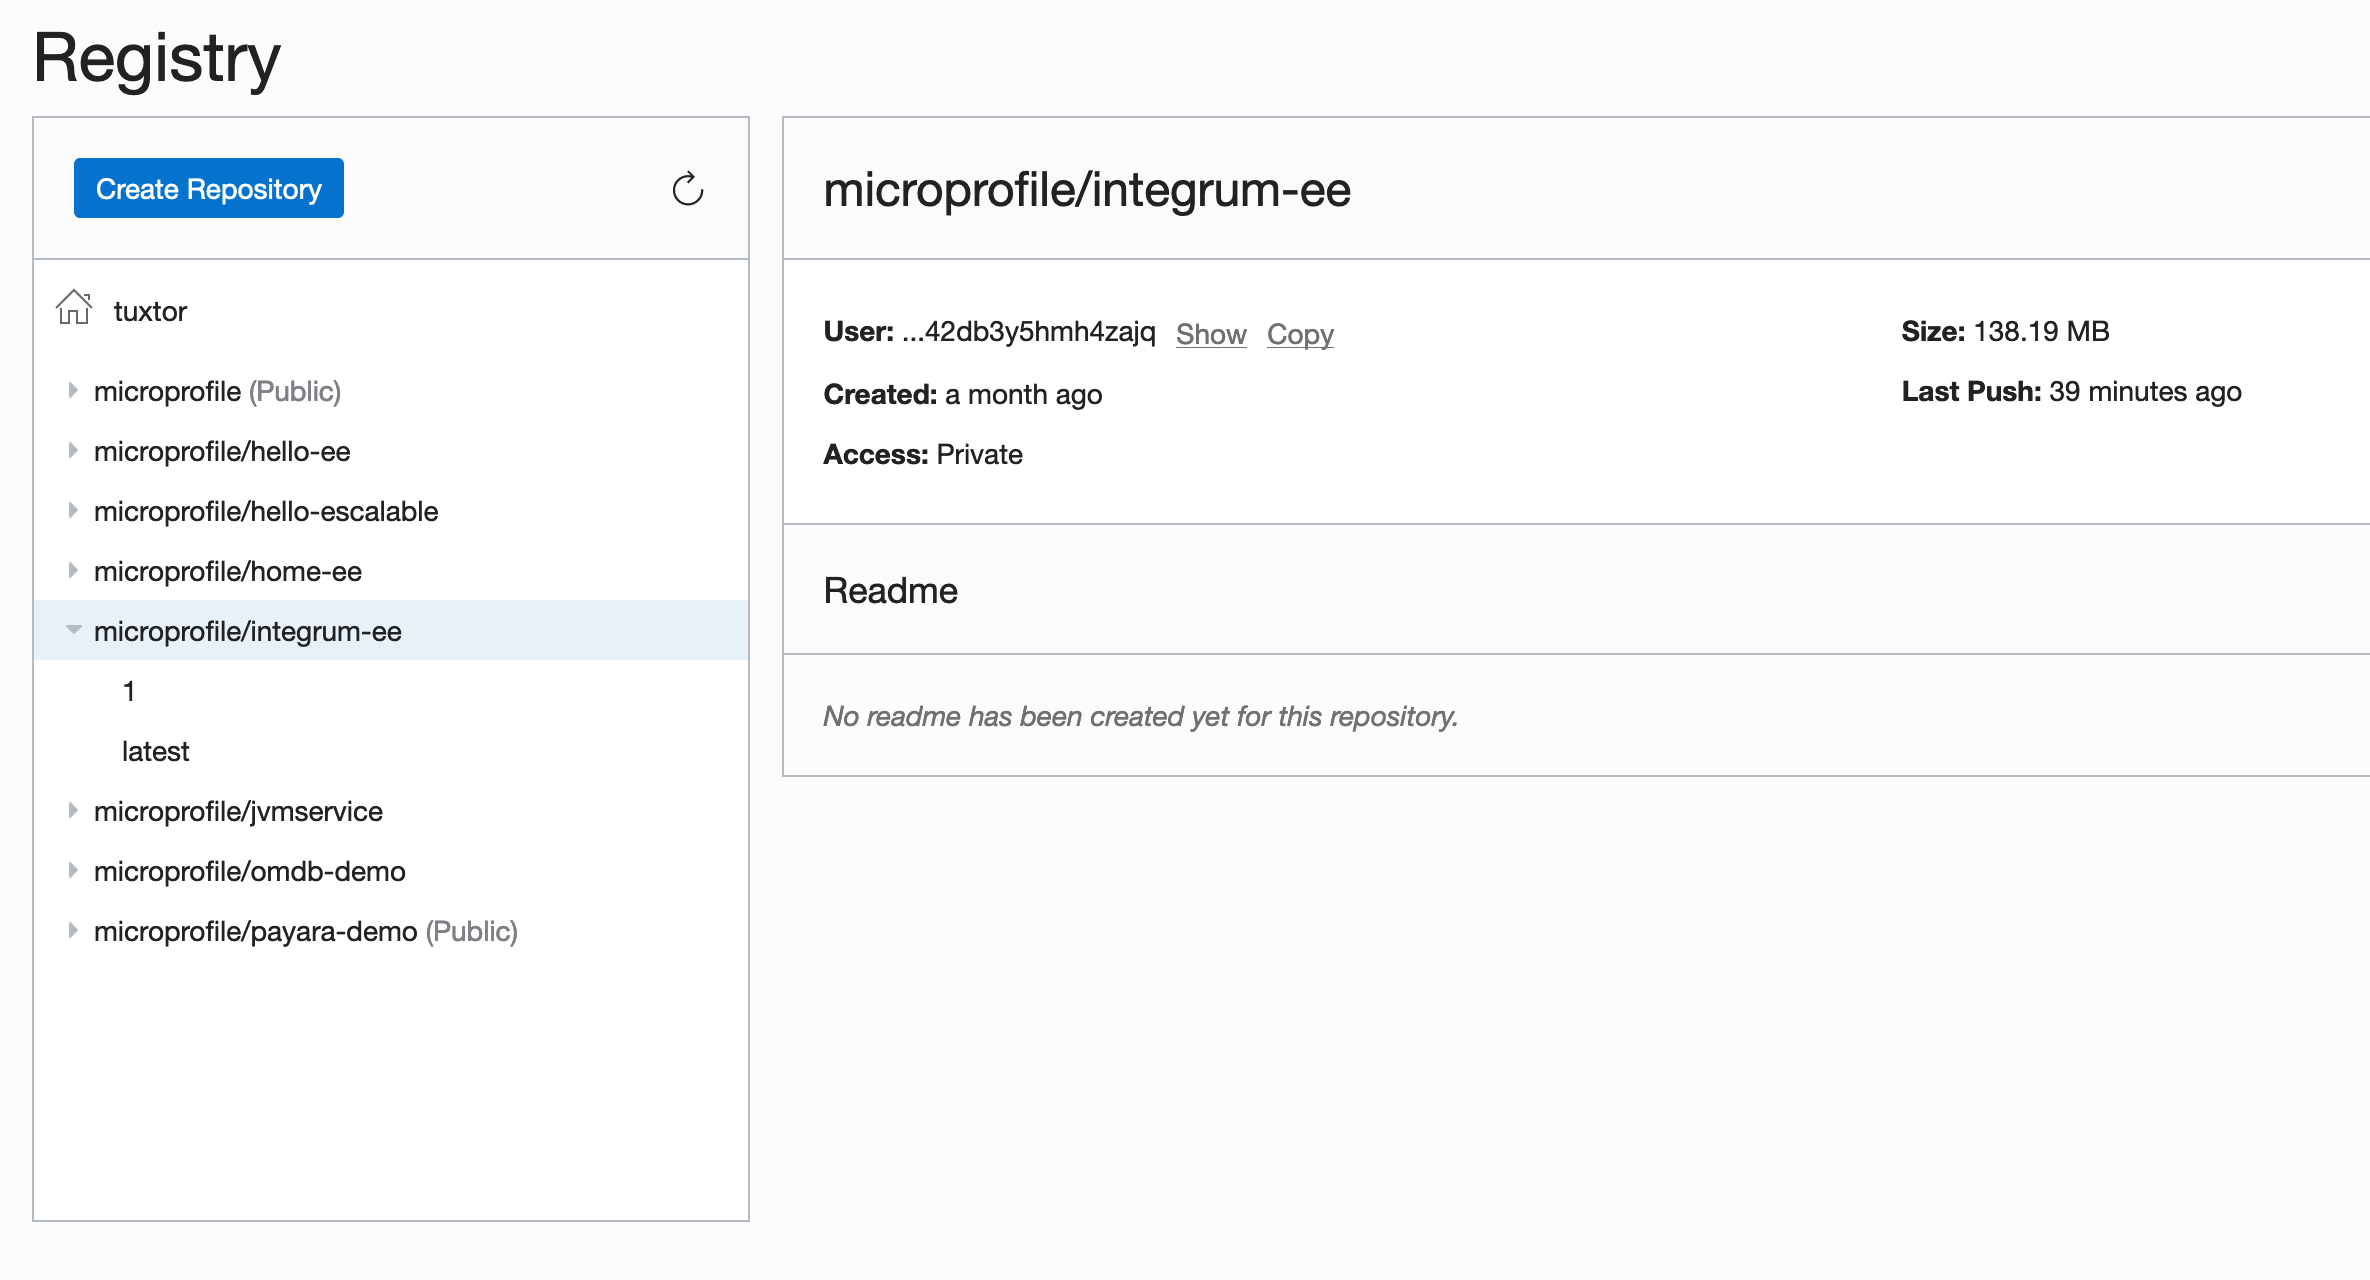
\includegraphics[width=0.95\linewidth]{Images/oc1}
\end{figure}
\end{frame}

\begin{frame}{Oracle Cloud}
\begin{figure}
	\centering
	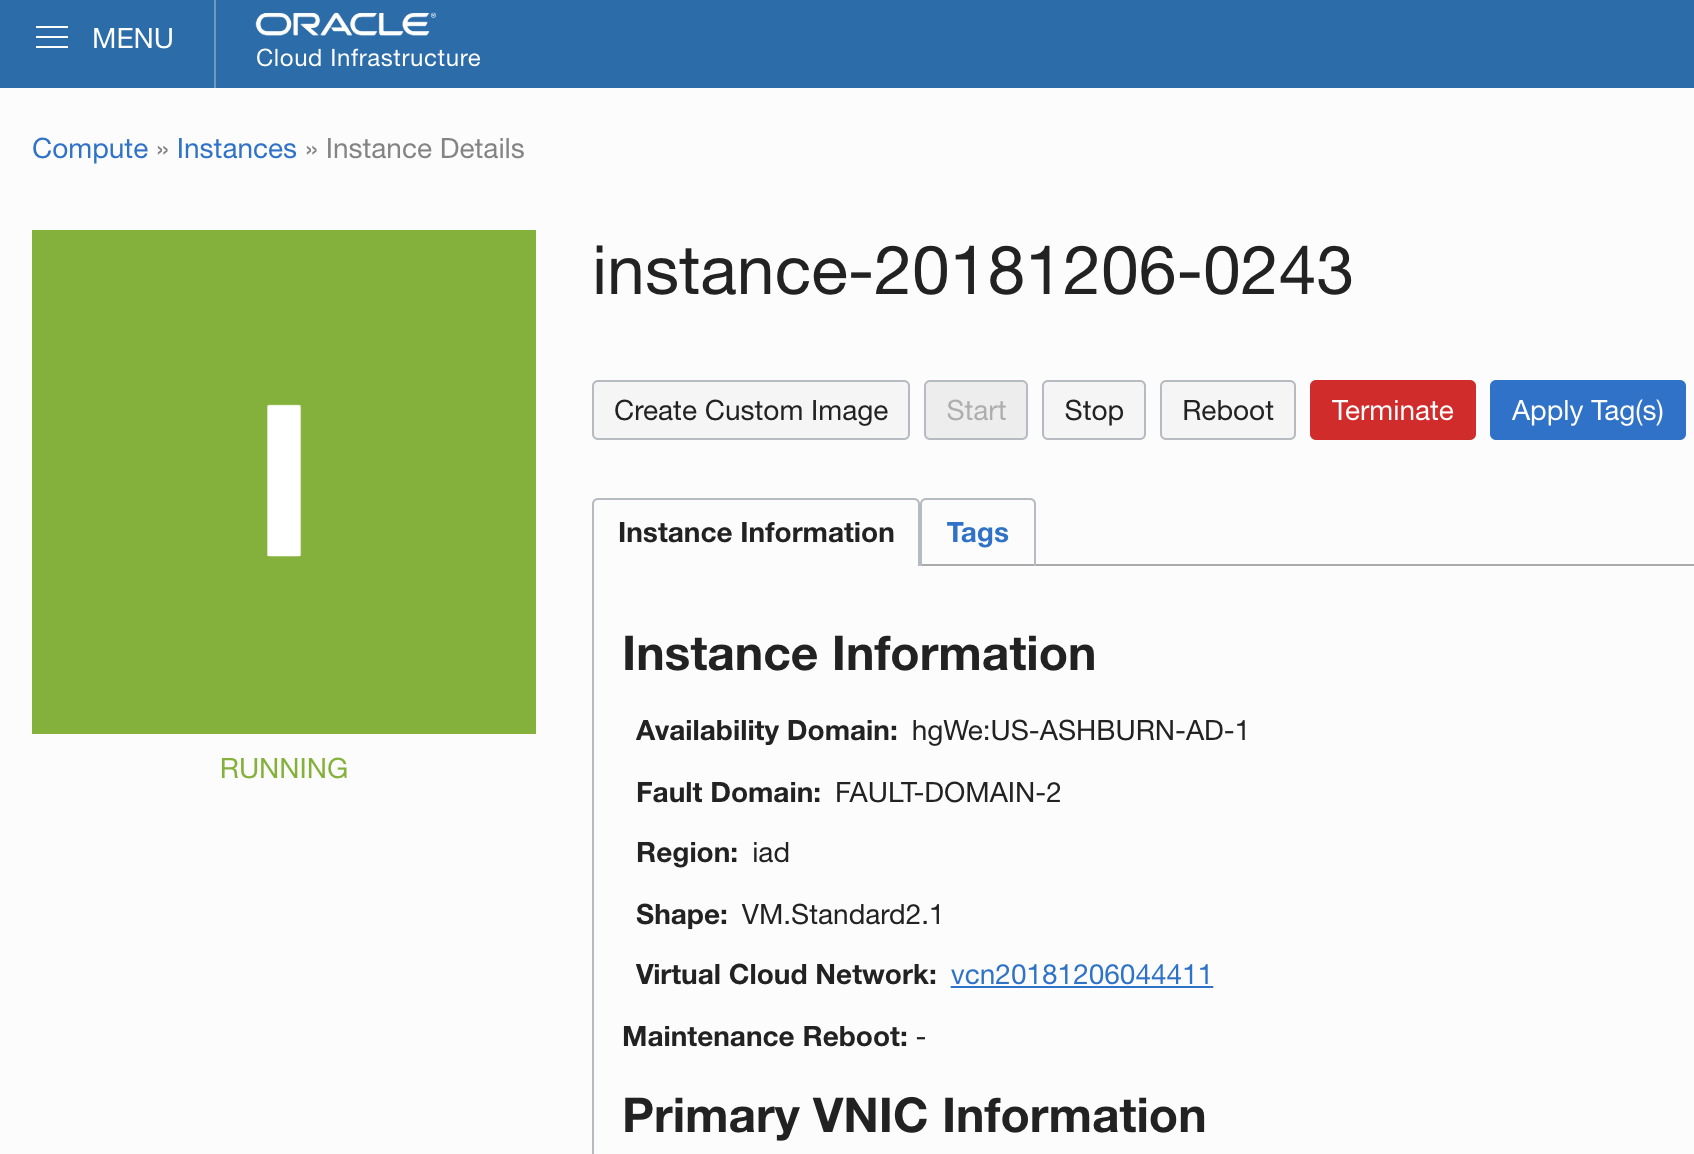
\includegraphics[width=0.95\linewidth]{Images/oc2}
\end{figure}
\end{frame}

\begin{frame}{Oracle Cloud}
\begin{figure}
	\centering
	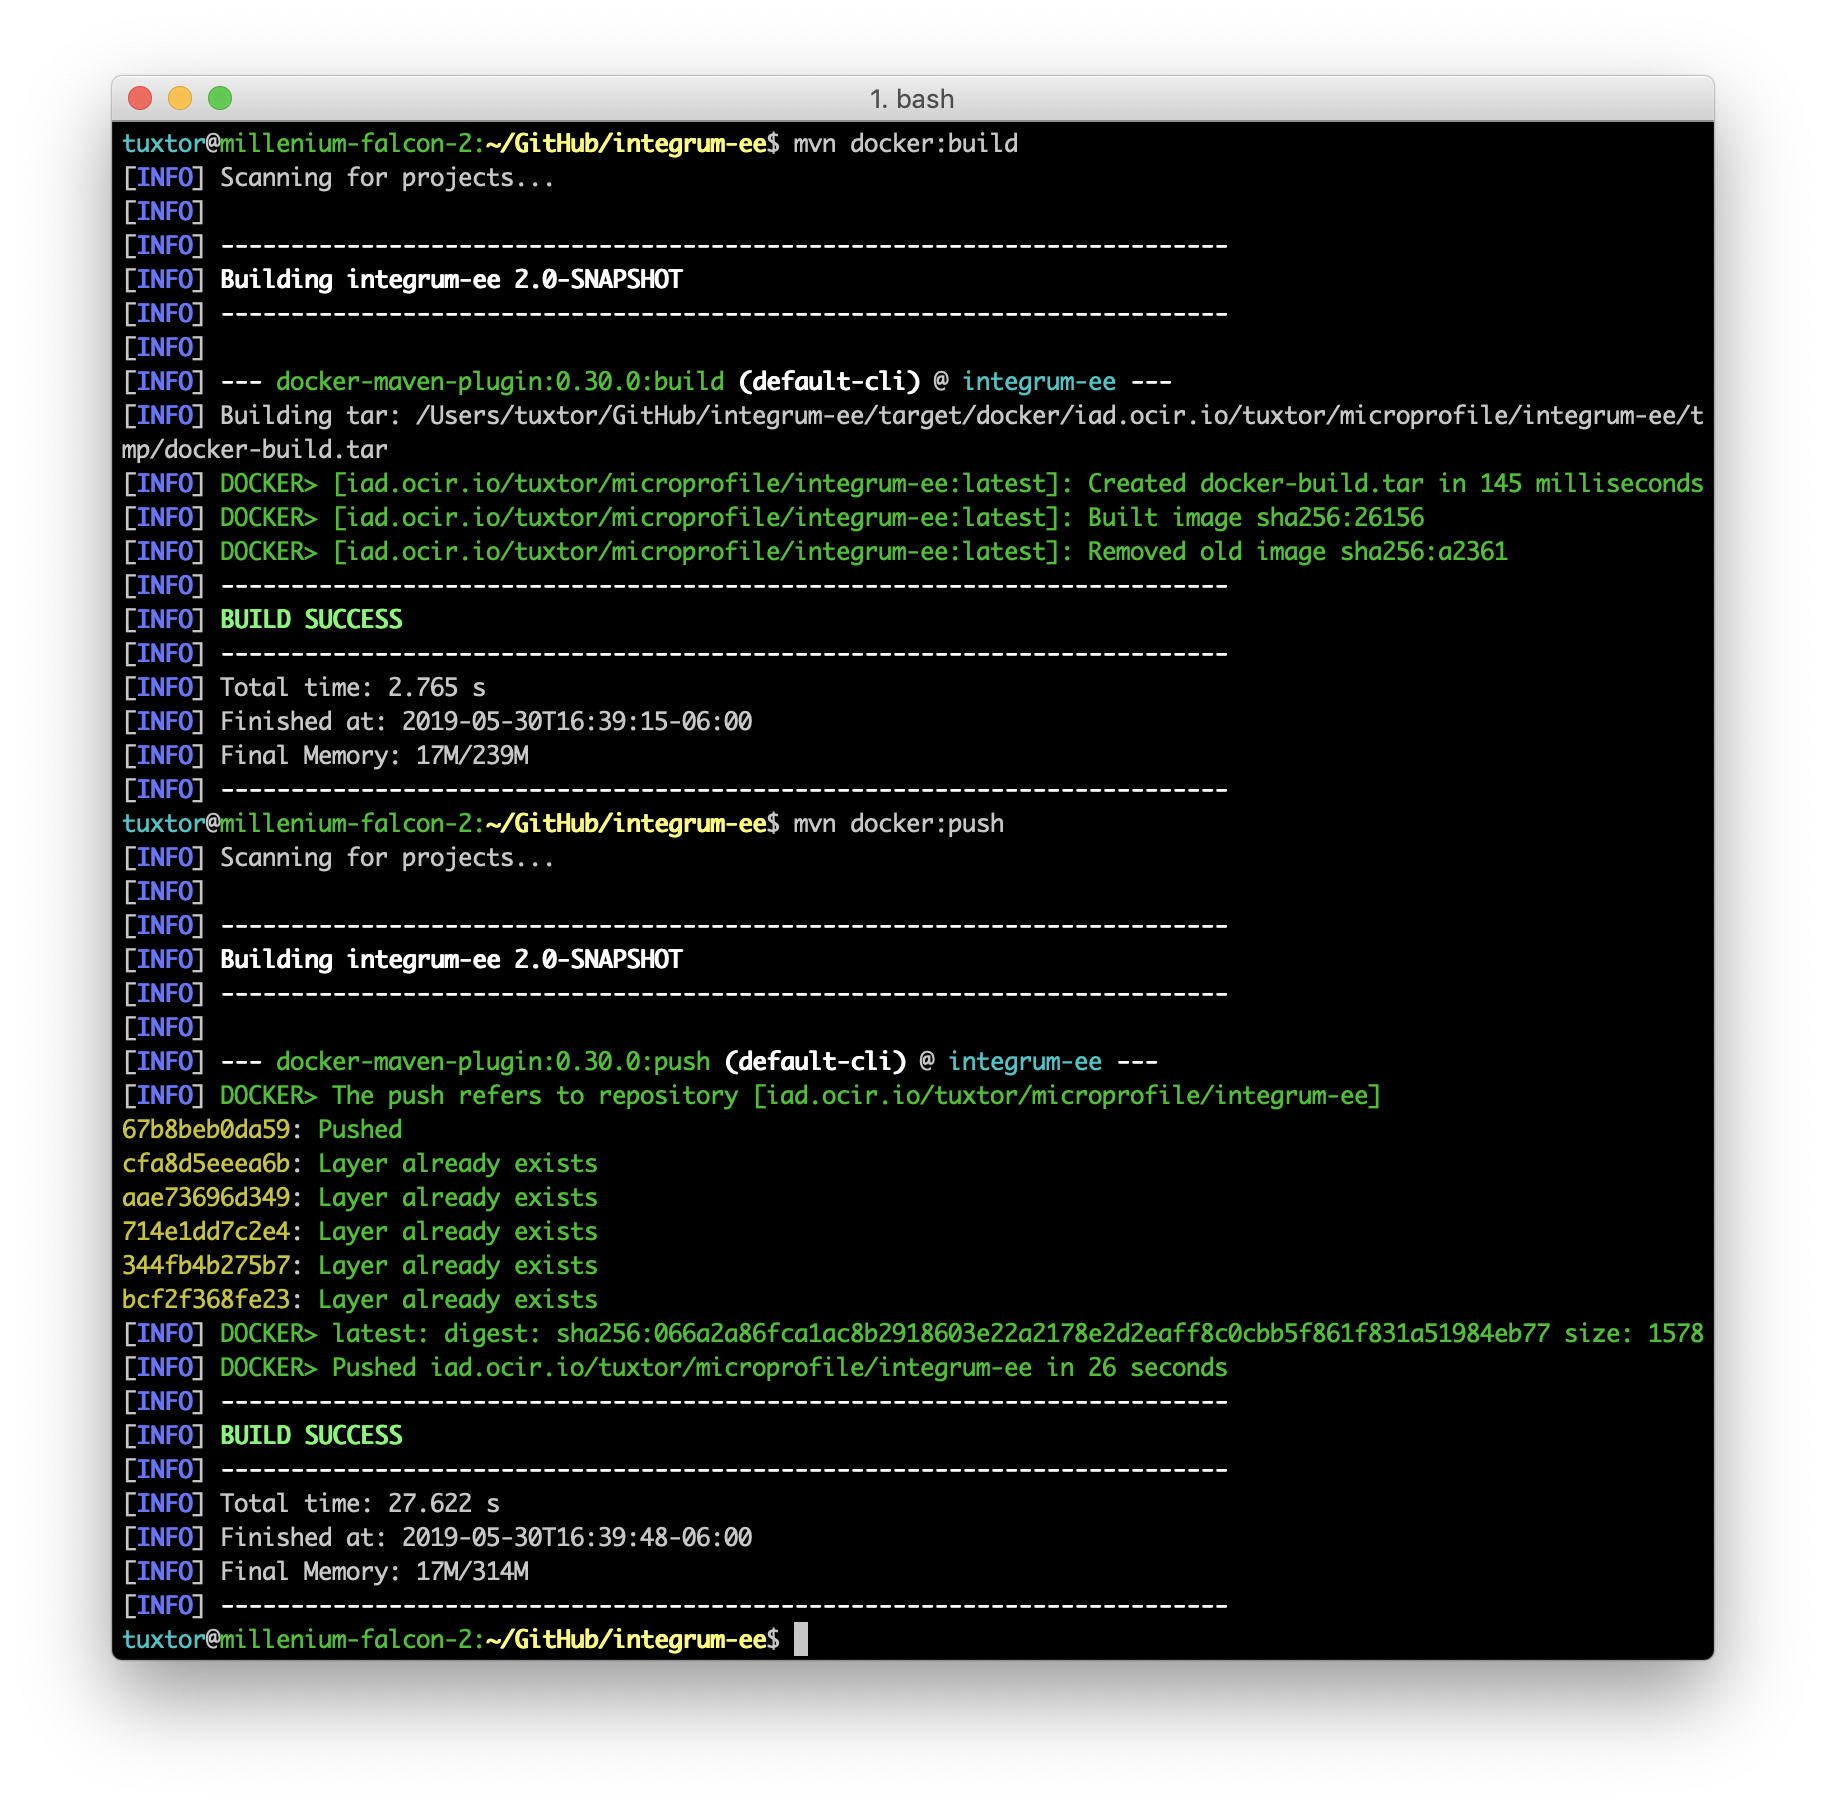
\includegraphics[width=\linewidth]{Images/oc3}
\end{figure}
\end{frame}

\begin{frame}{Oracle Cloud}

\begin{figure}
	\centering
	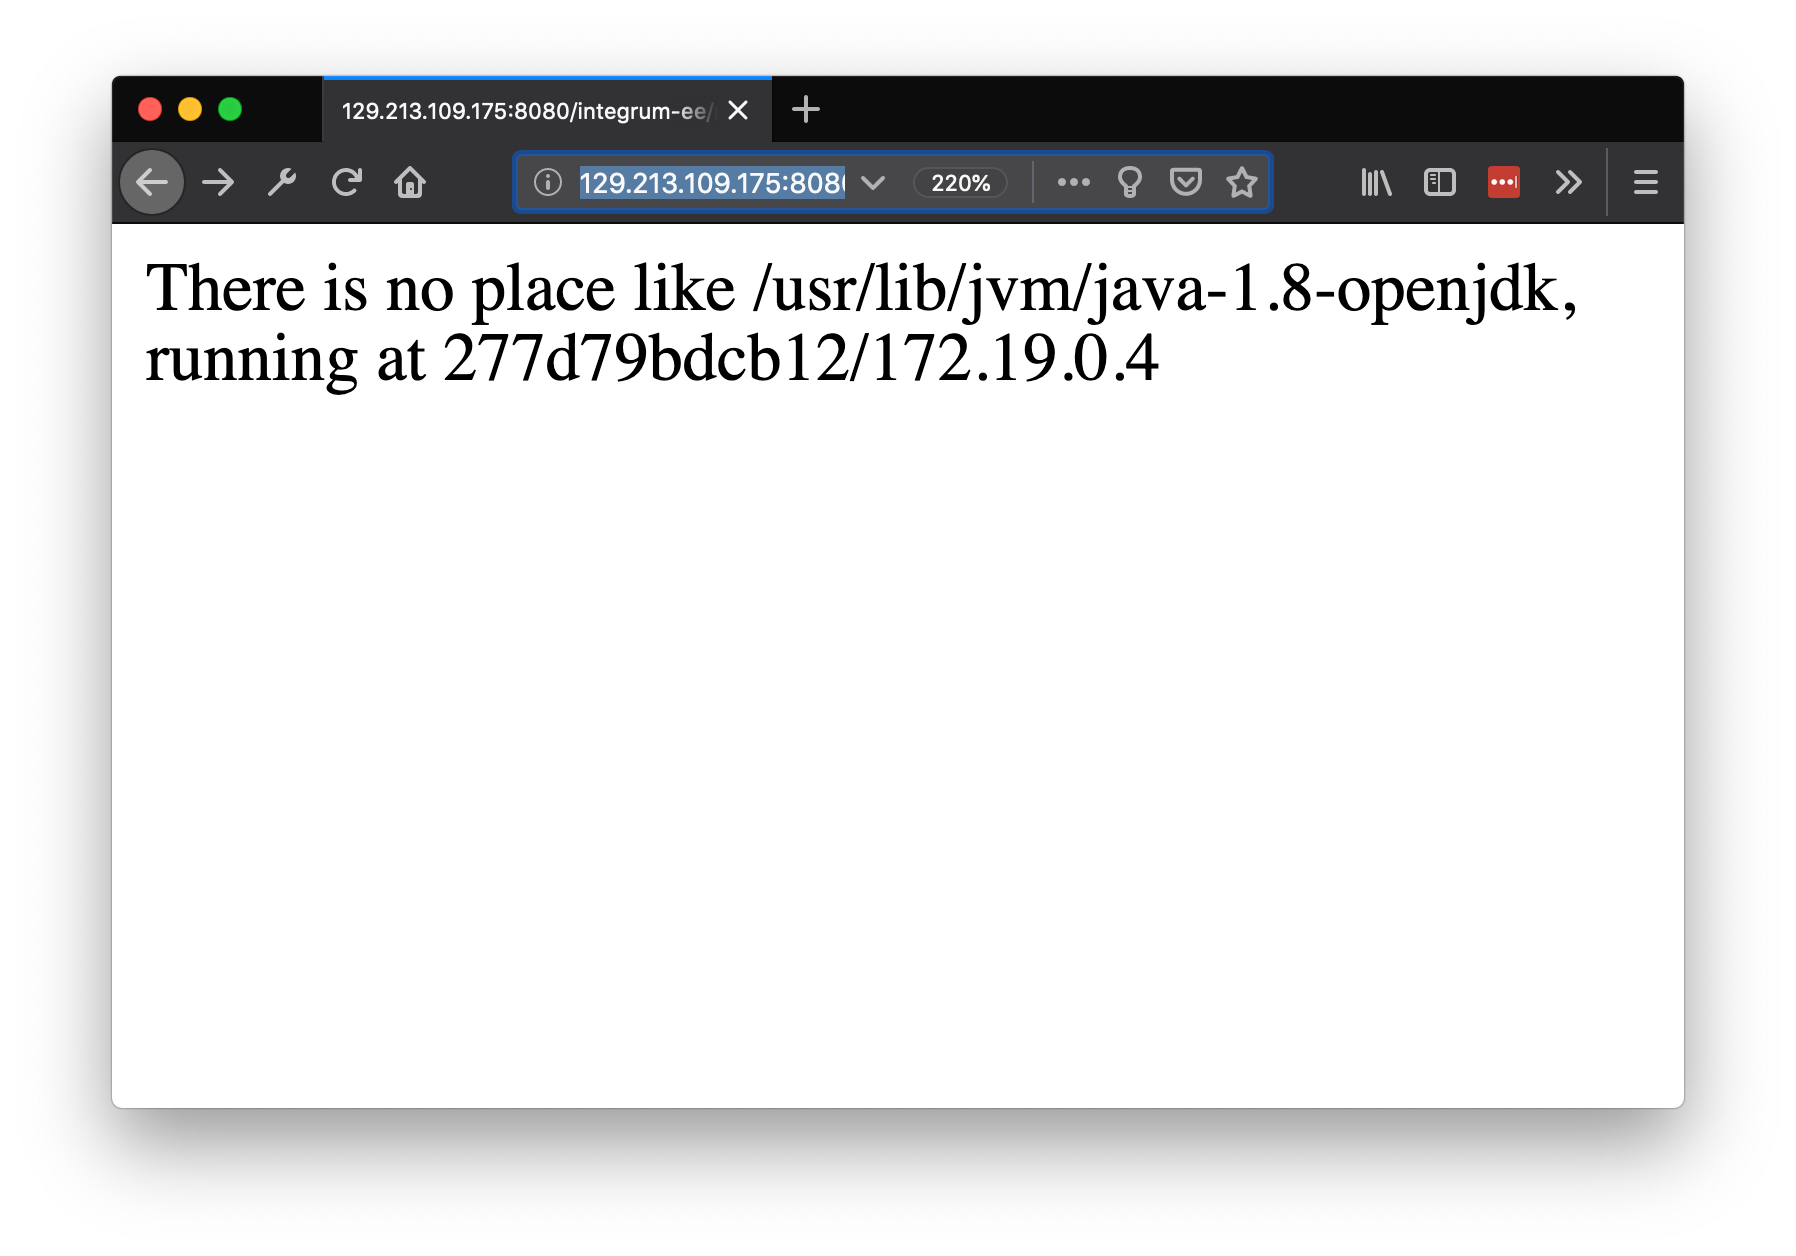
\includegraphics[width=\linewidth]{Images/oc4}
\end{figure}
\end{frame}



{
    \usebackgroundtemplate{
\includegraphics[width=\paperwidth]{Images/separador}}
    \setbeamercolor{normal text}{fg=white}
    \setbeamercolor{frametitle}{fg=red}
    \usebeamercolor[fg]{normal text}
    \section{Kotlin}
}

\begin{frame}{Kotlin}
\begin{columns}
	\begin{column}{0.5\textwidth}
		\begin{itemize}
			\item Static typing
			\item Java inter-op
			\item OO + FP
			\item Null safety
			\item Extension functions
			\item Operator overloading
			\item Data classes
			\item One line methods
		\end{itemize}
	\end{column}
	\begin{column}{0.5\textwidth}  %%<--- here
		\begin{figure}
			\centering
			
\includegraphics[width=0.7\linewidth]{Images/kotlin}
		\end{figure}
	\end{column}
\end{columns}
\end{frame}

\begin{frame}{Kotlin - Fatos interesantes}
\begin{columns}
\begin{column}{0.5\textwidth}
	\begin{itemize}
		\item Effective Java - Immutability, builder, singleton, override, final by default, variance by generics
		\item Elvis - Groovy
		\item Type inference - Scala
		\item Immutability - Scala
		\item Identifiers - Scala
		\item Null values management - Groovy
		\item Functions - Groovy
	\end{itemize}
\end{column}
\begin{column}{0.5\textwidth}  %%<--- here
	\begin{figure}
		\centering
		
\includegraphics[width=0.7\linewidth]{Images/kotlin}
	\end{figure}
\end{column}
\end{columns}
\end{frame}



\begin{frame}{Víctor Orozco}
\begin{columns}[T] % contents are top vertically aligned

	\begin{column}[T]{4cm} % alternative top-align that's better for graphics
		\begin{figure}
			\centering
			
\includegraphics[width=\linewidth]{Images/logos}
		\end{figure}
	\end{column}
	\begin{column}[T]{6cm} % each column can also be its own environment
		\begin{itemize}
			\item vorozco@nabenik.com
			\item \href{https://twitter.com/tuxtor}{@tuxtor}
			\item \href{http://www.nabenik.com}{https://vorozco.com}
		\end{itemize}
	\begin{center}
		
\includegraphics[width=0.1\linewidth]{Images/cclogo}
		\\
		This work is licensed under a Creative Commons Attribution-ShareAlike 3.0.
	\end{center}
	\end{column}
\end{columns}
\end{frame}


\end{document}